\chapter{METHODOLOGY}
\label{chap-three}

	EEG data for three different mental tasks were collected from four different test subjects. The three mental tasks are as shown in Table \ref{Tasks}. Each mental task was carried out for ten seconds and repeated five times comprising fifty seconds duration of EEG signal for each task. During each task the subjects were asked to sit on a chair, close their eyes and restrict any muscle movements. The raw EEG data collected from the EEG sensor was then passed through pre-processing block, feature extraction block and classifier block consecutively. Figure \ref{fig:FlowChart} shows the overall flow of data from the EEG sensors to classifier.
		\begin{figure}[hbtp]
            \centering
            \smartdiagram[priority descriptive diagram]{
                \centering
                EEG Sensor,
                Pre-processing (Filtering),
                Feature Extraction (Spectral Energy of EEG bands),
                Classification,
                Class Assignment}
    		\caption{Overview of User Verification System using EEG}
    		\label{fig:FlowChart}
    	\end{figure}
        
		\begin{table}[h]
			\centering
			\caption{Mental Tasks}
			\label{Tasks}
			\begin{tabular}{l l}
				\hline
				Task &Description\\\hline
				Calculating&Performing a mental calculation of two digit multiplication\\
				Breathing&Concentrating on breathing\\
				Singing&Mentally singing a song without actually singing out loud\\
			\end{tabular}
		\end{table}
    
    
\section{Pre-Processing}
	The data stream was read at 512 samples per second from MindWave Mobile EEG sensor and stored in a file. Different files were used for each user, each mental task and each repetition of the mental task. The stored raw EEG data was then passed through a band-pass filter to eliminate unnecessary frequency bands. If total number of samples for each repetition of a mental task for a given user was $n$, then the filtered data $X'=[x_1', x_2', \ldots, x_n']^T$ was obtained by passing $X=[x_1, x_2, \ldots, x_n]^T$ through the band pass filter $F$ as shown in Equation \ref{EQ:bpf}. The lower cutoff frequency and the higher cutoff frequency for the band pass filter were 0.1Hz and 48Hz respectively.
    
    \begin{equation}
		\label{EQ:bpf}
        X' = F(X) \;.
	\end{equation}
    
    The filtered data were then divided into subgroups, each subgroup with one second data. Say, if ten seconds of EEG readings were recorded, the total samples of raw EEG data stored in the file would be $512\times 10=5120$. Each sub group would contain $512\times1=512$ samples. And total number of sub groups would be $5120\div512=10$. Say, if EEG readings for user $i$ were collected for mental task $j$, repeated for $k^{th}$ time, then the filtered EEG data for sub group $l$ is given by Equation \ref{EQ:subGrp}.
    \begin{equation}
		\label{EQ:subGrp}
        X_{ijkl}' = [x_1', x_2', \ldots ,x_{511}', x_{512}']^T \;.
	\end{equation}
    
\section{Feature Extraction}
\label{FeatureExtraction}
	As discussed in Section \ref{EEG Frequency Bands} neural activities can be characterized by frequencies. Table \ref{Table:Bands} shows different EEG frequency bands and their frequency ranges. Since different brain activities result in different energy levels of EEG frequency bands, using spectral energy of EEG frequency bands as input feature vectors to the classifier is an excellent choice. In order to increase the dimension of input vectors, some of the EEG frequency bands were further sub-divided into low and high bands, resulting in eight EEG frequency bands as show in Table \ref{Table:Bands_more} (also see Figure \ref{fig:eeg_bands}).
    
    	\begin{table}[h!]
		\centering
		\caption{Frequency Bands used for Feature extraction}
		\label{Table:Bands_more}
		\begin{tabular}{l l}
			\hline
			Name &Frequency Band\\\hline
			Delta&0.1Hz - 4Hz\\
			Theta&4Hz - 8Hz\\
            Low Alpha&8Hz - 10Hz\\
			High Alpha&10Hz - 12Hz\\
            Low Beta&12Hz - 18Hz\\
			High Beta&18Hz - 30Hz\\
            Low Gamma&30Hz - 40Hz\\
			High Gamma&40Hz - 48Hz\\
		\end{tabular}
	\end{table}


	\begin{figure}[hbtp]
    	\centering
    	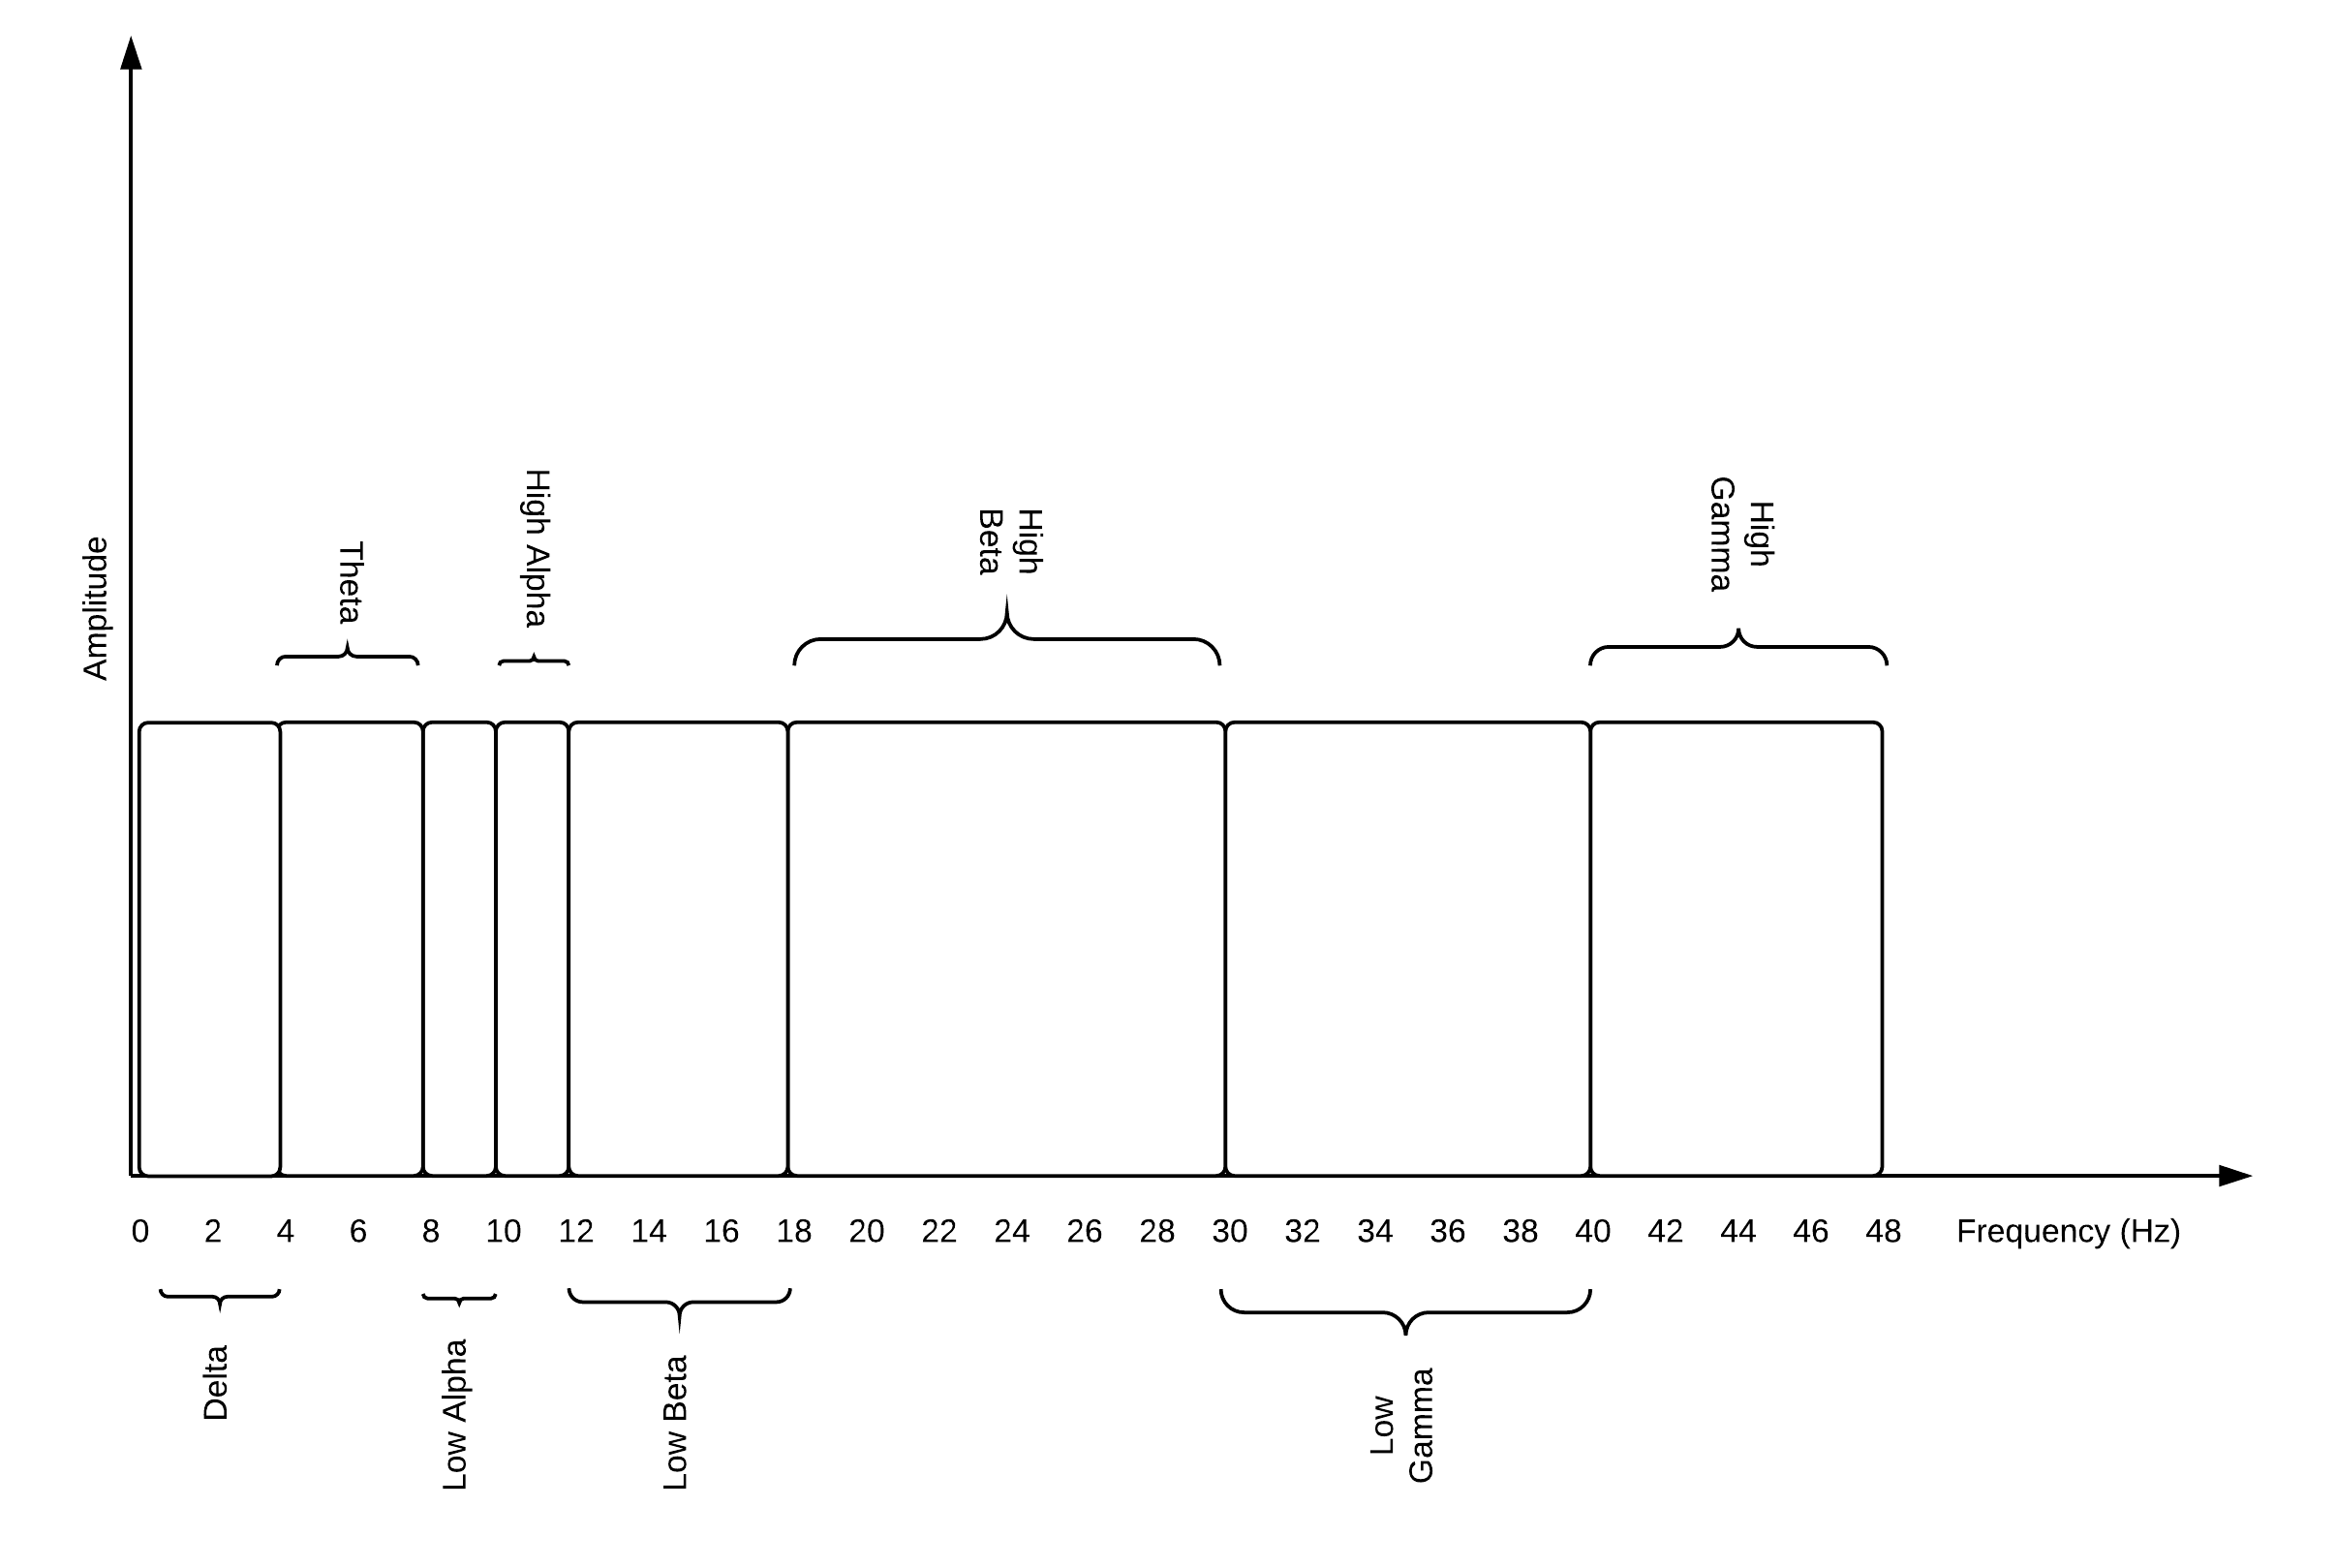
\includegraphics[width=1\textwidth]{Chapter-3/EEG_bands}
    	\caption{EEG Frequency Bands}
    	\label{fig:eeg_bands}
  	\end{figure}
    
	First, we pass the each subgroup of filtered EEG data(containing 512 samples) through the 512 point Discrete Fourier Transform (DFT) block and obtain their DFT.
    
    If $X(n)$ is the input data sequence, $\mathscr{F}$ is the DFT operation and $X_k$ is the DFT of $X(n)$, Equation \ref{EQ:time_to_dft} symbolically shows the DFT operation conducted on input sequence $X(n)$.
    
    \begin{equation}
    	X(n) \xrightarrow{\mathscr{F}} X_k \;.
        \label{EQ:time_to_dft}
    \end{equation}
    
    Say, if each subgroup of filtered EEG samples is $X(n) = [x_1, x_2, \ldots, x_{512}]^T$ and the DFT of $X(n)$ is $X(k)$, then the 512 point DFT of $X(n)$ is given by Equation \ref{EQ:dft}.
    
    
    \begin{equation}
    	X(k) = \sum_{n = 0}^{n = 511}{X(n) \cdot \exp{(-2 \pi i k n/512)}}, k \epsilon Z \;.
		\label{EQ:dft}
    \end{equation}
    
    The spectral energy of each EEG frequency band $i$ may be calculated using Equation \ref{EQ:spectral_energy}.
    
    \begin{equation}
    	E_i = \sqrt{\frac{1}{m_2 - m_1 + 1} \sum_{k=m_1}^{k=m_2} \left | X(k) \right | ^2} \;,
    	\label{EQ:spectral_energy}
    \end{equation}
    
    \noindent where $m_2$ > $m_1$ and $k=[m_1,m_2] \in $ EEG frequency band $i$.
    
    After obtaining the spectral energy of each EEG frequency band, we combine them to form a vector as shown in Equation \ref{EQ:in_vectors}.
    
    \begin{equation}
    	X_{in} = [E_1, E_2, \ldots E_8] \;.
    	\label{EQ:in_vectors}
    \end{equation}
    
    We then normalize the EEG spectral energy band vector $X_{in}$ as shown in Equation \ref{EQ:norm} to obtain an unit vector $X_{n}$. This is next used as the input for the classifiers discussed in Section \ref{Chap3:Classifiers}. Note that by normalizing, we were able to neutralize the effect of different sensitivity levels of EEG sensor for different users and test cases.
   
	\begin{equation}
    	X_{n} = \frac{1}{\left | X_{in} \right |} X_{in} \;.
    	\label{EQ:norm}
    \end{equation}
    
\section{Classifiers}
\label{Chap3:Classifiers}

		The input feature vectors obtained from the pre-processing block were randomly shuffled and split into training and testing. Following is the training and testing split percentage, 
		\begin{enumerate} 
			\item 70\% of the feature vectors data set were used as training set.
			\item 30\% of the feature vectors data set were used as testing set.
		\end{enumerate}
		For example, if each EEG mental task experiment (lasting 10 second each) is repeated 5 times, we have raw EEG data of 50 seconds. After pre-processing this data, we will have 50 input feature vectors. We then shuffle the ordering of these vectors and pick 35 (70\%) as part of training set and 15 (30\%) as part of testing set. The shuffling is done to randomize the training and testing split.
        
        Since we have different users performing many mental tasks, we can try to identify the mental task given the subject or we can try to identify the subject among many subjects given the mental task. For this reason, we have conducted two different types of classification as given below,
        
		\begin{enumerate}
			\item \textbf{Intra - Subject Classification} : Identifying a mental task in a set of mental tasks performed by a single subject.
			\item \textbf{Inter - Subject Classification} : Identifying a subject in a set of subjects performing the same mental task.
		\end{enumerate}
        
\subsection{Mahalanobis Distance}
\label{Mahalanobis Distance}
	As discussed in \ref{Chap2:Maha}, the Mahalanobis Distance is a simple pattern recognition technique used to identify the class of the input vector. In our case, a class is either the type of task or the subject performing the mental task depending on the the classification type. The input vector $\mathbf{x}$ is the pre-processed EEG data vector given by Equation \ref{EQ:chap3X}.

	\begin{equation}
    	\mathbf{x} = [x_1\quad x_2 \ldots x_N] \;,
    	\label{EQ:chap3X}
    \end{equation}
    \noindent where $N$ is the number of variable in the input vector $\mathbf{x}$.
	
    The Mahalanobis distance is computed using the Equation \ref{EQ:chap3Maha}.
	\begin{equation}
    	D^2_x = (\mathbf{x} - E[\mathbf{x}])^T \bm{\Sigma}^{-1} (\mathbf{x} - E[\mathbf{x}]) \;,
    	\label{EQ:chap3Maha}
    \end{equation}
    
    \noindent where $\bm{\Sigma} ^{-1}$ is the inverse of the covariance matrix $\Sigma$ and $E[\mathbf{x}]$ is the expected value of $\mathbf{x}$.
    
    The expected value of $\mathbf{x}$ is given by Equation \ref{EQ:chap3Mean}.

	\begin{equation}
		E[\mathbf{x}] = \bm{\mu} = [\mu_1 \mu_2 \ldots \mu_N] = \sum_{i=1}^{M}\mathbf{x}_i \;,
    	\label{EQ:chap3Mean}
    \end{equation}
    
    \noindent where M is the number of input vectors.
    
    The covariance matrix $\bm{\Sigma}$ is given by Equation \ref{EQ:chap3Cov}.
	\begin{equation}
		\bm{\Sigma} = [(E[\mathbf{x} - E[\mathbf{x}])(E[\mathbf{x} - E[\mathbf{x}])^T ]
    	\label{EQ:chap3Cov}
    \end{equation}    
    
 %   However, since estimate of all possible samples is not feasible, we compute the estimate of covariance %matrix using sample covariance matrix given by Equation \ref{EQ:chap3SampleCovEle}
 %   
 %   \begin{equation}
 %   	\bm{\Sigma} = \begin{bmatrix}
 %   				\Sigma_{11} & \Sigma_{12}  & \ldots & \Sigma_{1j} \\
 %   				\Sigma_{21} & \Sigma_{22}  & \ldots & x_{2j} \\
 %   				\vdots 	    & \vdots       & \ldots & \vdots\\
 %   				\Sigma_{i1} & \Sigma_{i2}  & \ldots & \Sigma_{ij}
%\end{bmatrix}
%    	\label{EQ:chap3SampleCov}
%    \end{equation}
%    
%    Here the sample covariance of each element i,j is computed as given in Equation 
%\ref{EQ:chap3SampleCovEle}
%   
%    \begin{equation}
%    	\bm{\Sigma}_{ij} = \frac{1}{N} \sum_{k=1}^{N} (F_i(k) - \mu_i)(F_j(k) - \mu_j)
%    	\label{EQ:chap3SampleCovEle}
%    \end{equation}
%    
%    where $N$ is the number of samples in feature $F_i$ and $\mu_i$ is given by Equation 
%\ref{EQ:chap3SampleMean}.
%   
%    \begin{equation}
%		\mu_i = \frac{1}{N} \sum_{k=1}^N F_i(k)
%    	\label{EQ:chap3SampleMean}
%    \end{equation}    
    
    As discussed in \ref{Chap2:Maha}, we first calculate the mean vectors and sample covariance matrices for all the classes in the training set. We then calculate the Mahalanobis distance of the input testing vector with respect to each and every class using their corresponding mean vector and sample covariance matrix. We then assign the class label to the input testing vector by computing ``the class which gives smallest Mahalanobis distance''. Say, if we have class $C_1, C_2 \ldots , C_m$ and $d_1, d_2 \ldots d_m$ are the corresponding Mahalanobis distances of an input testing vector, we assign this input vector the class label $C_i$, if $d_i = min(d_1, d_2 \ldots , d_m)$. Similarly, we then classify every single input in the testing set using Mahalanobis Distance.  
    
\subsection{Artificial Neural Networks}
\label{Artificial Neural Networks}
 
 	In Section \ref{Chap2:ANN}, we briefly discussed Artificial Neural networks and how they can be used in pattern recognition. In this section, we will discuss perceptrons and multiple layer feed forward neural network.
    
    \subsubsection{Perceptron}
    
    \begin{figure}[hbtp]
    	\centering
    	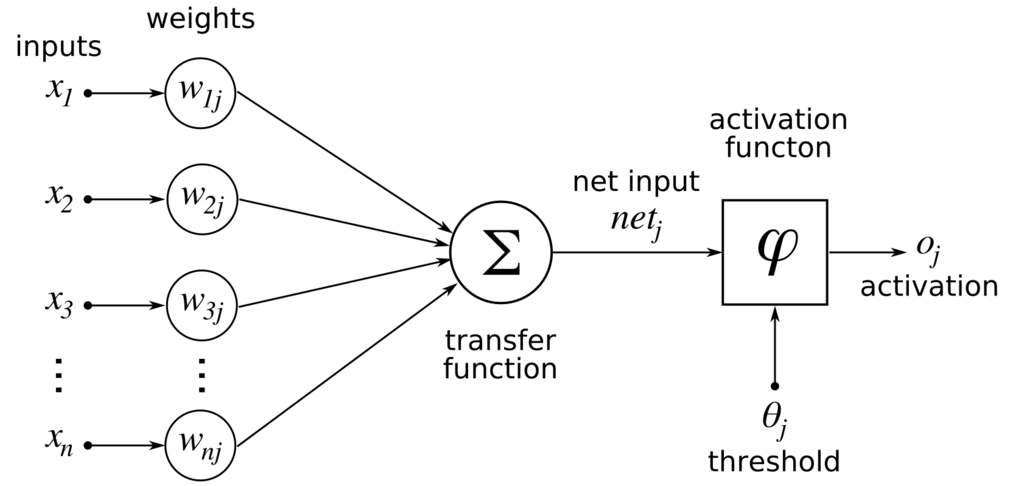
\includegraphics[width=0.9\textwidth]{Chapter-2/ann}
    	\caption{Perceptron \cite{aneuronimage}}
    	\label{fig:chap3ann}
    \end{figure}
    
    Consider Figure \ref{fig:chap3ann}, where input $\bm{x}$ and weights of the perceptron $\mathbf{w}$ are given by Equation \ref{EQ:chap3input} and Equation \ref{EQ:chap3weights} respectively. Perceptron uses the input vector $\mathbf{x}$ and weight vector $\mathbf{w}$ such that the classification boundary, $\mathbf{w}^T\mathbf{x} = 0$ separates the classes.
    
    
    \begin{equation}
    	\mathbf{x} = [1 x_1 x_2 x_3 \ldots x_m]^T \;.
        \label{EQ:chap3input}
    \end{equation}    
	\begin{equation}
    	\mathbf{w} = [w_0 w_1 w_2 \ldots w_m]^T \;.
        \label{EQ:chap3weights}
    \end{equation}

	The output of the perceptron for a given input vector is calculated using Equation \ref{EQ:chap3PerOut}.
    
    \begin{equation}
    	F(\mathbf{x}) = \varphi(\mathbf{w}^T\mathbf{x}) \;,
		\label{EQ:chap3PerOut}
    \end{equation}
        
	\noindent where $\varphi$ is the activation function. Different activation function like tanh (Equation \ref{EQ:chap3tanh}), sigmoid (soft step) (Equation \ref{EQ:chap3softstep}) etc., can be used as activation function. The choice of the activation function does not affect the training methods. For our experiments we use sigmoid activation function.
    
    \begin{equation}
    	\varphi(v) = \frac{e^v - e^{-v}}{e^v + e^{-v}} \;.
    	\label{EQ:chap3tanh}
    \end{equation}
    \begin{equation}
		\varphi(v) = \frac{1}{1 + e^{-v}} \;.
    	\label{EQ:chap3softstep}
    \end{equation}        
        
        
        Since the perceptron is a supervised machine learning algorithm, it requires training. Here, the training involves tuning the weight vector $\mathbf{w}$. This can be done using the Gradient Decent algorithm. If $d_j$ represents the desired output and $y_j$ is the actual output of the perceptron for $j^{th}$ input vector $x_j$, we can calculate the error function for $i^{th}$ iteration of the gradient decent algorithm using Equation \ref{EQ:chap3Grad}.
        
        \begin{equation}
        	E^{(i)} = \frac{1}{2m}\sum_{k =1}^{k = m} (\varphi(\mathbf{w}^T x(k)) - d(k))^2 \;.
        	\label{EQ:chap3Grad}
        \end{equation}
        
        The Gradient Decent Algorithm states that, the error function $E$ can be minimized (given that $\varphi(\mathbf{w}^T x(k))$ is differentiable) by updating the weight vector as shown in Equation \ref{EQ:chap3GradUpdate}.
        
        
        \begin{equation}
        	\mathbf{w}^{(i + 1)} = \mathbf{w}^{(i)} - \eta \cdot \mathbf{x} \cdot (\mathbf{y}^{(i)} - \mathbf{d}) \;,
        	\label{EQ:chap3GradUpdate}        
        \end{equation}
        
        \noindent where $\mathbf{y} = [y_1 y_2 \ldots y_n]^T$ is the actual output of the perceptron in vector form, $\mathbf{d} = [d_1 d_2 \ldots d_n]^T$ is the desired output of the perceptron in vector form and $\eta$ is the learning rate parameter. The learning rate parameter $\eta$ determines how fast the weights converge. Keeping $\eta$ too low will result in slow convergence resulting in large number of iterations to reach the optimal solution. On the other hand, large $\eta$ might not guarantee the optimal solution. Hence, it is better to start $\eta$ with a high value and gradually reduce it after every iteration.
        
        \subsubsection{Multi Layer Perceptron}
        
        The Multi layer perceptron (MLP) is an extension of the perceptron. This architecture has more neurons connected to each other and allows  non-linear classification boundaries. As discussed in Section \ref{Chap2:ANN}, the multi layer perceptron typically contains an input layer, one or more hidden layers and an output layer as shown in Figure \ref{fig:chap3mult} . 

    \begin{figure}[hbtp]
    	\centering
    	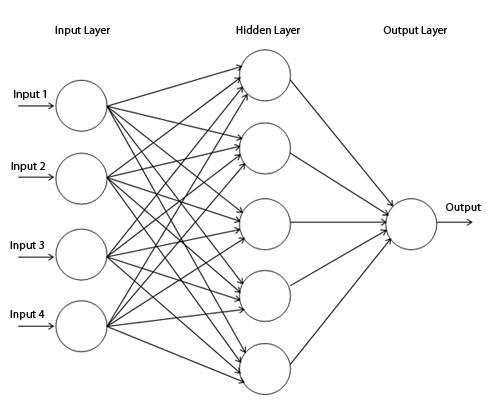
\includegraphics[width=0.9\textwidth]{Chapter-3/mult}
    	\caption{Multi Layer Perceptron \cite{multipercep}}
    	\label{fig:chap3mult}
    \end{figure}
    
        According to Universal approximation theorem, a single hidden layer with finite number of neurons is sufficient to approximate a given training set \cite{simonHaykin}. Hence, a single hidden layer was used for our use case. Also, The Sigmoid (soft step) (Equation \ref{EQ:chap3softstep}) function was used as the activation function. The features used for the Neural Network are as shown in Table \ref{NN_features}.
        
		\begin{table}[h!]
			\centering
			\caption{Neural Network Features}
			\label{NN_features}
			\begin{tabular}{l l}
				\hline
				Parameters &Value\\\hline
				Type of network &Feed Forward network\\
				Input layer size &8\\
				No. of hidden layers &1\\
				Hidden layer size &8\\
                Output layer size &Vary based on number of classes\\
				Activation function in hidden layer &Sigmoid\\
                Training Algorithm used &Backpropagation Algorithm
			\end{tabular}
		\end{table}
        
        Just like the perceptron, the MLP has a input vector $\mathbf{x} = [1 x_1 x_2 \ldots x_{m_{0}}]^T$ of dimension $m_0 + 1 \times 1$. Here, $x_0 = 1$ is the bias term. Similar to the perceptron, the MLP also has weights. Since we have multiple neurons in the hidden layer connected to the input layer, we instead have a weight matrix $\mathbf{w}$ with dimension $(m_0 + 1) \times m_1$, given by Equation \ref{EQ:chap3weightMatrix}.
        
        
        \begin{equation}
        	\mathbf{w} = \begin{bmatrix}
        		w_{10}^{(1)} 	&w_{20}^{(1)} \ldots 	& w_{m_{1}0}^{(1)} \\
        		w_{11}^{(1)} 	&w_{21}^{(1)} \ldots 	& w_{m_{1}1}^{(1)} \\
            	\vdots     	&\vdots    			& \vdots \\
        		w_{1m_{0}}^{(1)} &w_{2m_{0}}^{(1)} \ldots &w_{m_{1}m_{0}}^{(1)} \\
        	\end{bmatrix} \;.
        	\label{EQ:chap3weightMatrix}
        \end{equation}
       
       Here the subscript in $w_{ij}^k$, $i$ and $j$ represent the connection from $j^{th}$ input to the $i^{th}$ neuron in the hidden layer. The superscript $k$ represent the $k^{th}$ hidden layer. Since only one hidden layer was used, we have $k = 1$. Each column vector in the matrix $\mathbf{w}$ represents the weight vector for a single neuron in the hidden layer. The output of the hidden layer is calculated using Equation \ref{EQ:chap3hiddenOut}.
       
       
       	\begin{equation}
       		\mathbf{x}_{h_0} = \varphi(\mathbf{w}^T \mathbf{x}) \;,
       		\label{EQ:chap3hiddenOut}
       	\end{equation}
        
        \noindent where $\varphi$ is the activation function.
        
        The output of hidden layer is then used as the ``input' to the output layer. After adding a bias term to the output of the hidden layer, we have $\mathbf{x}_{h{1}}$ given by Equation \ref{EQ:chapnn3h1}.
        
        
        \begin{equation}
        	\mathbf{x}_{h_1} = [1\quad \mathbf{x}_{h_0}]^T \;.
        	\label{EQ:chapnn3h1}
        \end{equation}
        
        Output of the network is then calculated using Equation \ref{EQ:chap3nnout}.
        \begin{equation}
       		y(\mathbf{x}) = \varphi(\mathbf{w_o}^T \mathbf{x}_{h_1}) \;,
        	\label{EQ:chap3nnout}
        \end{equation}        
        
        \noindent where $\mathbf{w}_o$ is is given by Equation \ref{EQ:chap3weightMatrixout}.

        \begin{equation}
        	\mathbf{w}_{o} = \begin{bmatrix}
        		w_{10}^{(2)} 	&w_{20}^{(2)} \ldots 	& w_{m_{2}0}^{(2)} \\
        		w_{11}^{(2)} 	&w_{21}^{(2)} \ldots 	& w_{m_{2}1}^{(2)} \\
            	\vdots     	&\vdots    			& \vdots \\
        		w_{1m_{1}}^{(2)} &w_{2m_{1}}^{(2)} \ldots &w_{m_{2}m_{1}}^{(2)} \\
        	\end{bmatrix} \;,
        	\label{EQ:chap3weightMatrixout}
        \end{equation}
        
        \noindent where $m_1$ is the number of neurons in the hidden layer and $m_2$ is the number of neurons in the output layer.
        
        
        Training the neural network was done using backpropagation algorithm. Backpropagation algorithm is an iterative algorithm, which minimizes the output error by adjusting the weight matrices of the network. The detailed description of backpropagation algorithm can be found in \cite{duda2001pattern}.
        
\subsection{Support Vector Machines (SVMs)}
\label{Support Vector Machines}
	As discussed in Section \ref{chap2:SVM} the SVMs maximize the distance between the separating hyperplane and the nearest points of the classes to the hyperplane. The detailed derivation of how SVMs achieve this can be found in \cite{snyder2010machine}. The the results in sections \ref{Linear SVM} and \ref{Nonlinear SVM} follow the detailed derivation of SVMs in \cite{snyder2010machine}.
    
    \subsubsection{Linear SVMs}
    \label{Linear SVM}
    If $i^{th}$ input vector is given by $\mathbf{x_i} = [x_1 x_2 \ldots x_m]$, then the objective function $L(\mathbf{\lambda)}$ of the SVM is given by Equation \ref{EQ:chap3svmObj}.
    
    \begin{equation}
    	L(\bm{\lambda)} = \sum_{i = 0}^{N} \lambda_i - \frac{1}{2} \sum_{i = 1}^{N} \sum_{j = 1}^{N} \lambda_i \lambda_j y_i y_j \mathbf{x}_i^{T} \mathbf{x}_j.
    	\label{EQ:chap3svmObj}
    \end{equation}
    
    \begin{equation}
    	\sum_{i = 1}^{N} \lambda_i y_i = 0.
    	\label{EQ:chap3const1}
    \end{equation}
    
    \begin{equation}
    	\lambda_i \geq 0, i = 1, \ldots ,n.
    	\label{EQ:chap3const2}
    \end{equation} 
    
	Here, $y_i$ is the desired output for the $i^{th}$ input sample. The goal here is to find the Lagrange multipliers $\alpha_i's$, so that the objective function $L(\bm{\lambda)}$ is maximized. Also, while optimizing the objective function, the constraints shown in Equation \ref{EQ:chap3const1} and Equation \ref{EQ:chap3const2} are used given the training data. This is called the ``dual form'' of the constrained optimization problem of the support vector machines. Also, all the input vectors in the training set with $\alpha_i \neq 0$ are called the ``support vectors'' (hence the name).
    
    By defining matrix $A$ as shown in Equation \ref{EQ:chap3MatrixA} and if $\Lambda$ denotes the vector of Lagrange multipliers, we can write the matrix form of $L(\mathbf{\lambda})$ as shown in Equation \ref{EQ:chap3lagMatrixForm} \cite{snyder2010machine}.
    
   	\begin{equation}
    	A = 
    	\begin{bmatrix}
	    	y_i y_j \mathbf{x}_i^T \mathbf{x}_j
    	\end{bmatrix}.
   		\label{EQ:chap3MatrixA}
   	\end{equation}
   
    
    \begin{equation}
    	L(\bm{\lambda)} = - \frac{1}{2} \Lambda^T A \Lambda + \mathbf{1}^T \Lambda,
    	\label{EQ:chap3lagMatrixForm}
    \end{equation}
    
   \noindent where $\mathbf{1}$ is a vector of all ones. After finding the required Lagrange multipliers, we can compute the optimal projection vector using Equation \ref{EQ:chap3OptimalProj}.
    
    \begin{equation}
    	\mathbf{w} = \sum_i \lambda_i \mathbf{x}_i y_i\; ,
    	\label{EQ:chap3OptimalProj}
    \end{equation}
    
    \noindent where $y_i$ is given by Equation \ref{EQ:chap3yi},
    \begin{equation}
    	y_i = (\mathbf{w}^T \mathbf{x} + b)
    	\label{EQ:chap3yi}
    \end{equation}
    
    \noindent and $b$ can be solved using Equation \ref{EQ:chap3b},
    
    \begin{equation}
    	\lambda_i(y_i(\mathbf{w}^T \mathbf{x}_i +b) - 1) = 0 \forall i.
    	\label{EQ:chap3b}
    \end{equation}
    
    \subsubsection{Nonlinear Support Vector Machines}
        \label{Nonlinear SVM}
    	Here, we apply nonlinear transformation $\bm{\vartheta}$ to the input vector $\mathbf{x}_i$ to produce a vector of higher dimension $\mathbf{x}_{i}'$ as shown in Equation \ref{EQ:chap3nonLinTrans}.
    
    \begin{equation}
    	\mathbf{x}_{i}' = \bm{\vartheta}(\mathbf{x}_i) : (\mathbb{R}^d \rightarrow \mathbb{R}^m), m > d.
    	\label{EQ:chap3nonLinTrans}
    \end{equation}
    
    Now, if we apply Equation \ref{EQ:chap3nonLinTrans} to Equation \ref{EQ:chap3MatrixA}, we have,
    
    \begin{equation}
		A = 
    	\begin{bmatrix}
	    	y_i y_j \bm{\vartheta}(\mathbf{x}_i)^T \bm{\vartheta}(\mathbf{x}_j)
    	\end{bmatrix}.
    	\label{EQ:chap3Amod}
    \end{equation}
    
    The nonlinear operation and the inner product can be replaced by the single operation called ``Kernel function'' $\mathbf{K(a,b)}$ if it satisfies the following Mercer's condition,
    
	\begin{equation}
		\int \mathbf{K(a,b)} g(\mathbf{a}) g(\mathbf{b}) \  d\bm{a} \  d\bm{b} \geq 0 \;,
        \label{EQ:chap3mercerscondition}
	\end{equation}

    \noindent where $g(\mathbf{x})$ has finite energy. One of the most popular kernel which satisfies the Mercers condition is the Radial Basis Function given by Equation \ref{EQ:chap3RBF}.
    
    \begin{equation}
    	\mathbf{K}(\mathbf{a}, \mathbf{b}) = \textmd{exp}\left( - \frac{(\mathbf{a} - \mathbf{b})^T (\mathbf{a} - \mathbf{b})}{2\sigma^2}\right).
    	\label{EQ:chap3RBF}
    \end{equation}
    
    
    \section{Conclusion}
    
    In Chapter \ref{chap-three}, we discussed the User Verification System using EEG signals pipeline in detail. We discussed about how to collect the data from Mindwave Mobile EEG sensor, how to pre-process the raw EEG signals to remove noise, how to extract feature vectors from pre-processed EEG signal, how to classify the input feature vectors using Mahalanobis distance, Neural Networks and SVMs. In next chapter, we will discuss about the results of classification.
    
    
    
    
    
    
    
    
    
    
    
    
    
    
    
    
    